\documentclass{article}
\usepackage{graphicx} % Required for inserting images
\usepackage{graphicx} % Required for inserting images
\usepackage[ngerman]{babel}
\usepackage{enumitem}
\usepackage{float}
\usepackage{chngcntr}
\usepackage{glossaries}
\usepackage{tabularx}
\usepackage{hyperref}
\usepackage{titletoc}
\counterwithin{figure}{section}
\counterwithin{table}{section}
\setlength\parindent{0pt}

\makeglossaries

\newglossaryentry{Attributsableitung}
{
    name=Attributsableitung,
    description={Besteht aus einem Namen und einer Ableitung aus existierenden Spalten der Tabelle oder anderen Attributsableitungen.}
}

\newglossaryentry{Alternative}
{
    name=Alternative,
    description={Ein alternatives Verkehrsmittel im Modell. Besteht aus einem Namen und einer Nutzenfunktion, die i.Allg. Referenzen auf Attribute oder Attributsableitungen besitzt.}
}

\newglossaryentry{Projektdatei}
{
    name=Projektdatei,
    description={Enthält potentiell eine CSV-Datei, sowie eventuell Attributsableitungen, Alternativen und vorherige Ergebnisse.}
}

\newglossaryentry{Valide Attributsableitung}
{
    name=Valide Attributsableitung,
    description={Eine Attributsableitung, dessen Name eindeutig ist, die syntaktisch korrekt ist und dessen Referenzen auf Attribute alle existieren.}
}

\newglossaryentry{Invalide Attributsableitung}
{
    name=Valide Attributsableitung,
    description={Eine Attributsableitung, dessen Name bereits vorkommt, die syntaktisch inkorrekt ist oder die eine Referenz auf ein nicht-existierendes Attribut hat.}
}

\newglossaryentry{Valide Alternative}
{
    name=Valide Alternative,
    description={Eine Alternative, dessen Name eindeutig ist, dessen Nutzenfunktion syntaktisch korrekt ist und dessen Referenzen auf Attribute alle existieren.}
}

\newglossaryentry{Invalide Alternative}
{
    name=Invalide Alternative,
    description={Eine Alternative, dessen Name bereits vorkommt, dessen Nutzenfunktion syntaktisch inkorrekt ist oder die eine Referenz auf ein nicht-existierendes Attribut hat.}
}

\newacronym{Ableitung}{Ableitung}{Attributsableitung}

\newacronym{WK}{WK}{Wunschkriterium}

\newacronym{CSV}{CSV}{Comma-separated values}

\newacronym{JSON}{JSON}{JavaScript Object Notation}


\title{Entwurf \\ \large Discrete Choice Model Builder}
\author{Kevin Boehnke \\ \texttt{uxpkw@student.kit.edu}
\and Floriane Bresser \\ \texttt{uspvq@student.kit.edu}
\and Damian Reich \\ \texttt{uqppn@student.kit.edu}
\and Alissa Saleh \\ \texttt{unmbc@student.kit.edu}
\and Michael Schur \\ \texttt{ufkmz@student.kit.edu}}
\date{23. Juni 2023}

\begin{document}

\maketitle
\newpage
\startcontents[maintableofcontents]
\printcontents[maintableofcontents]{}{1}[2]{\section*{Inhaltsverzeichnis}}
\thispagestyle{empty}
\newpage
\pagenumbering{arabic}

\section{Einleitung}


\section{Paketstruktur}
\begin{figure}[H]%
    \centering
    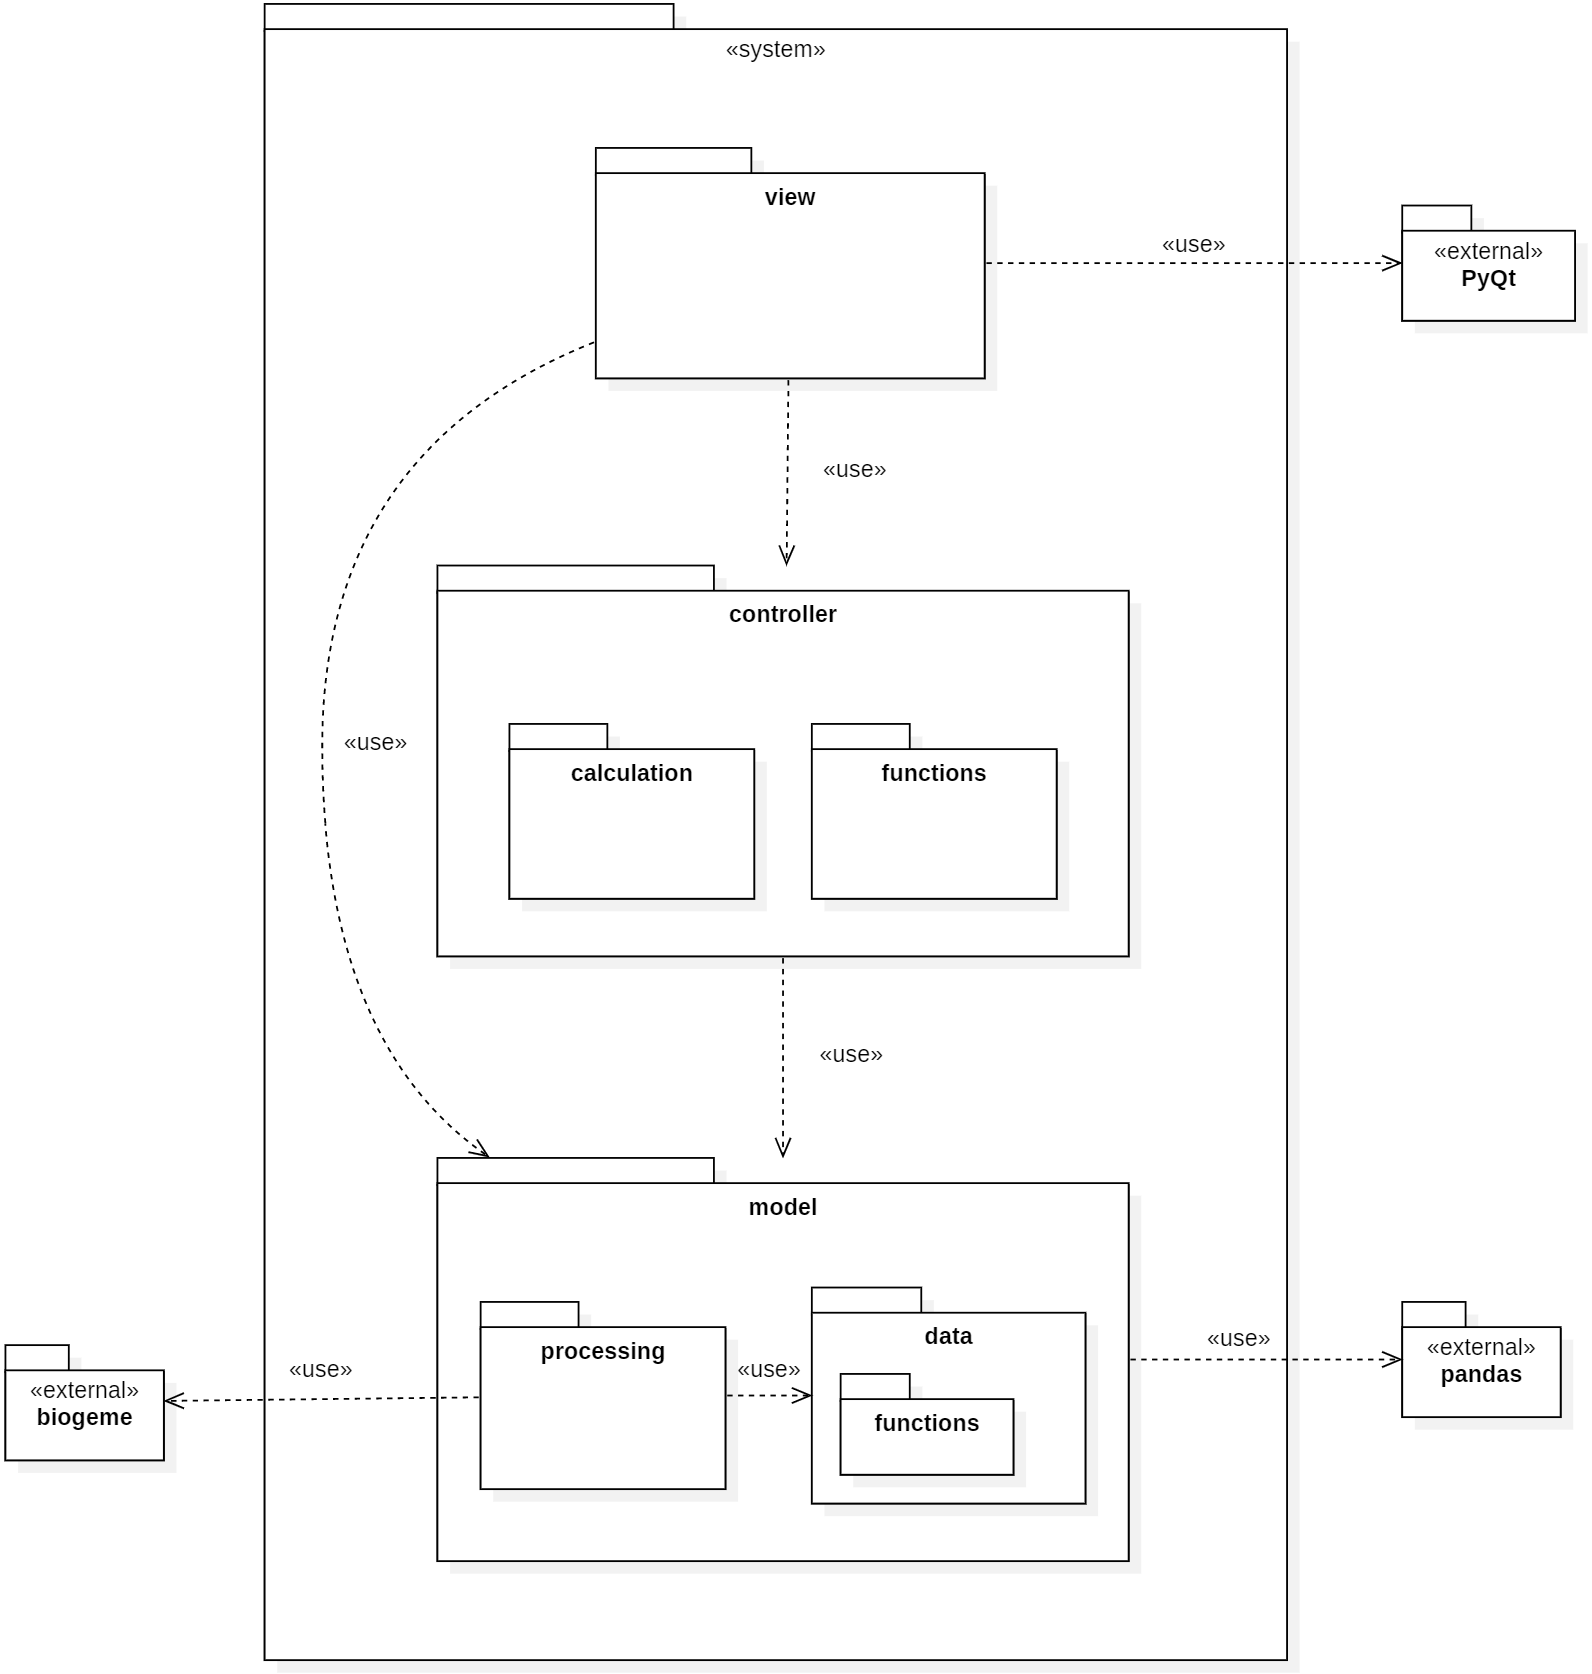
\includegraphics[width=13cm]{img/PackageDiagram.png}
    \caption{Paketdiagramm}
\end{figure}

- Die Software ist eine MVC-Architektur und setzt sich zusammen aus der View, dem Controller und dem Model.
\subsection{View}
- Die View ist verantwortlich für die visuelle Präsentation der im Model vorhandenen Daten. Dafür greift die View auf das externe Paket PyQt zu, welches für die Erstellung graphischer Benutzeroberflächen verwendet wird.
\subsection{Controller}
- Die Controller sind dafür zuständig, die Nutzereingaben aus der View an das Model weiterzuleiten.\\
- Finden Änderungen am Model statt, so senden die betroffenen Klassen der View update-Aufrufe über die Controller aus. Dabei werden die Daten im Model zurückgegeben.\\
- Calculation-Paket: Controller, die für die gesamte Funktionalität der Berechnung aufgerufen werden\\
- Functions-Paket: Controller, die für die Bearbeitung von Alternativen und Attributsableitungen aufgerufen werden
\subsection{Model}
- Das Model umfasst die Datenhaltung bei einem geöffneten Projekt. \\
- Bei Änderungen ist das Model zudem verantwortlich vergangene Eingaben zu speichern. Diese sollen anhand einer undo-/redo-Funktion wieder aufrufbar sein.\\
- Processing-Paket: Umschließt die Funktionalität, welche mit der Konfiguration der Berechnung oder dem Ergebnis zu tun hat. Hier existiert eine Schnittstelle, über welche die tatsächliche Berechnung stattfinden kann. Hier wird standardmäßig das Python Paket \textit{biogeme} verwendet. \\
- Data-Paket: Bezieht alle Klassen mit ein, die für die Datenhaltung des Modells zuständig sind. \\
- Das Python Paket \textit{pandas} wird für die Haltung tabellarischer, vom Nutzer nicht veränderbarer Daten verwendet.


\section{Klassenstruktur}
\subsection{View}
\subsection{Model}
\newpage
\subsection{Controller}

Im folgenden Abschnitt werden die Klassen des Paketes 'Controller' so wie sie in Abb.X dargestellt sind dokumentiert.

\begin{figure}[H]%
    \centering
    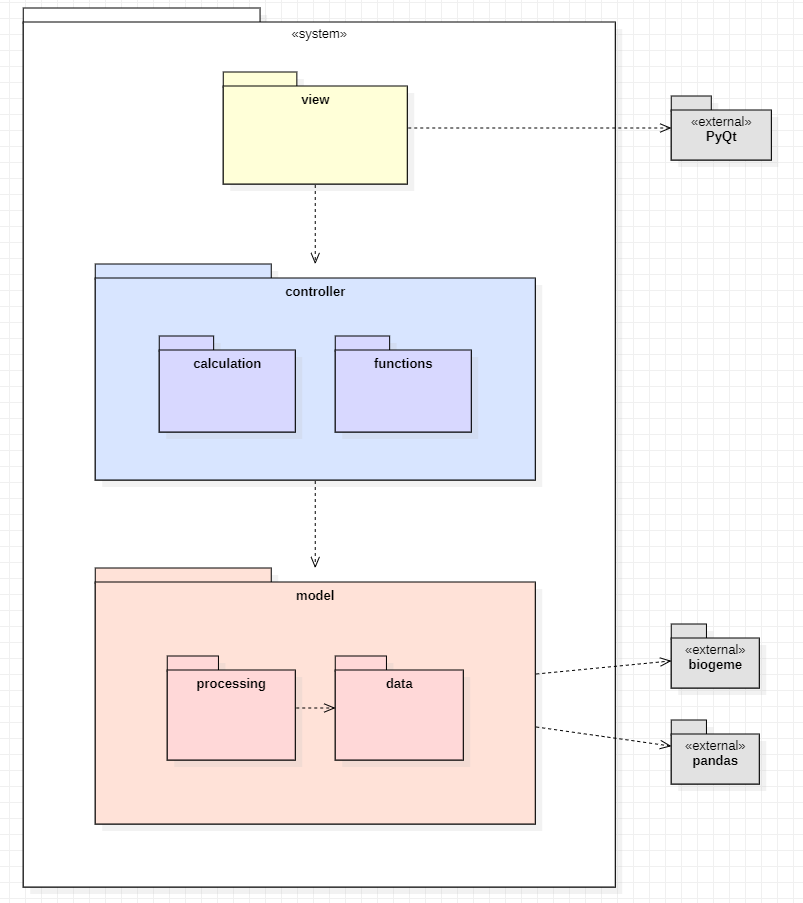
\includegraphics[width=13cm]{img/Floriane/PackageDiagram.png}
    \caption{Paketdiagramm}
\end{figure}


\newpage
\textbf{\large{FileManager}}\\\\
Abbildung XY

Das Interface \textit{FileManager} dient der Interaktion mit externen Dateien. Es wird von allen Klassen im Controller implementiert.
\newline \newline
\textbf{{Methoden}}
\begin{itemize}
\item \texttt{import(path:str):bool} \newline Dient dem Import aller notwendigen Dateien und behandelt den Zugriff auf diese. Die Controller implementieren die Methode um sie für die jeweiligen Daten bzw. Funktionen zu nutzen.
\\\\
\underline{{Parameter}}

\begin{tabular}{lll}
 & \texttt{path:str} & Der Pfad zum Speicherort der zu importierenden Datei. \\
\end{tabular}

\underline{{Rückgabewert}}

\begin{tabular}{lll}
 & \texttt{bool} & Ob der Export erfolgreich war. \\
\end{tabular}


\item \texttt{export(path:str):bool} \newline Führt den Export einer Datei zu einem bestimmten Pfad aus. Diese Methode wird vom jeweiligen Controller implementiert.
\\\\
\underline{{Parameter}}

\begin{tabular}{lll}
 & \texttt{path:str} & Der Pfad zum Speicherort der zu speichernden Datei. \\
\end{tabular}

\underline{{Rückgabewert}}

\begin{tabular}{lll}
 & \texttt{bool} & Ob der Export erfolgreich war. \\
\end{tabular}
\end{itemize}

\section{Softwareablauf}
- sequenz und aktivitätsdiagramme
\subsection{Projektmanagement}
\subsection{Attributsmanagement}
\subsection{Alternativmanagement}
\subsection{Konfiguration}
\subsection{Evaluation}


\section{Datenhaltung}

Der Model Builder speichert fünf verschiedene Ergebnisse: Alternativen, Attributsableitungen, Signifikanzen und Parameter, sowie die csv-Datein mit den zugrunde liegenden Umfragedaten und berechneten Attributen. Dabei werden Alternativen und Attributsableitungen im JSON-Format gespeichert, sodass sie in anderen Projekten widerverwertet werden können.

\subsection{Alternativen}
Die Alternativen werden als JSON Dateien mit ihren Attributen 'label' und 'functional\_expression' gespeichert. Zusätzlich wird ebenfalls das Erstellungsdatum gespeichert.

\newline
\{ \newline
    "label: string", \newline
    "functional\_expression": {\newline
        \texttt{"}expression": string, \newline
    }, \newline
\} \newline
\newline

Das Label wird als String gespeichert und dient der Unterscheidung der einzelnen Alternativen. Das Objekt der FunctionalExpression, das im Builder verwendet wird, wird unter 'functional\_expression' als Objekt mit seinen Attributen gespeichert. In diesem befindet sich die von Python evaluierbare Funktion unter "expression", inklusive möglicher nicht-behobener Fehler.

\subsection{Attributsableitungen}
Die Attributsableitungen werden ebenfalls separat als Funktion in einer JSON-Datei gespeichert. In den Dateien befinden sich die Schlüssel 'label' und 'functional\_expression'. Der Schlüssel 'label' enthält den gewählten Namen der Attribtusableitung, und 'functional\_expression' enthält das Objekt aus dem Projekt im JSON-Format. Dieses enthält den Funktionasausdruck als String unter dem Schlüssel 'expression'.

\newline
\{ \newline
    "label: string", \newline
    "functional\_expression": {\newline
        \texttt{"}expression": string, \newline
    }, \newline
\} \newline
\newline


\subsection{Umfragedaten und berechnete Attribute}
Die Umfragedaten werden auf Wunsch mit den berechneten Attributen in einer gemeinsamen csv-Datei gespeichert. 

Dabei entsprechen die Zeilen jeweils einer berechneten Attributsableitung. Die Spaltenüberschriften entsprechen den gesetzten Namen der Attributsableitungen. 

\subsection{Parameter und Signifikanzen}
Die berechneten Parameter und Signifikanzen werden in einer csv-Datei unter ihrem zugehörigen Variablen Namen gespeichert. Jede Zeile entspricht einer Variable aus den Nutzenfunktionen.

Die Spaltenüberschriften sind 'P' für die Spalten die Parameter enthalten und 'X' für die Spalten die die Signifikanzen enhalten. 

Die erste Spalte in der Tabelle enthält die durch die Nutzenfunktoinen festgelegten Variablennamen.


\section{Änderungen im Pflichtenheft}
- edit menu fehlt (nur undo, redo das ganze Projekt, Copy und Paste usw nur text)
- Speicherung nicht mehr zeitlich geregelt sondern schrittweise


\end{document}
